%% LyX 2.3.2 created this file.  For more info, see http://www.lyx.org/.
%% Do not edit unless you really know what you are doing.
\documentclass[english,aspectratio=169,handout]{beamer}
\usepackage{mathptmx}
\usepackage{eulervm}
\usepackage[T1]{fontenc}
\usepackage[latin9]{inputenc}
\usepackage{babel}
\usepackage{amsmath}
\usepackage{amssymb}
\usepackage{asymptote}
\usepackage{graphicx}
\ifx\hypersetup\undefined
  \AtBeginDocument{%
    \hypersetup{unicode=true,pdfusetitle,
 bookmarks=true,bookmarksnumbered=false,bookmarksopen=false,
 breaklinks=false,pdfborder={0 0 0},pdfborderstyle={},backref=false,colorlinks=true,
 allcolors=NYUPurple,urlcolor=LightPurple}
  }
\else
  \hypersetup{unicode=true,pdfusetitle,
 bookmarks=true,bookmarksnumbered=false,bookmarksopen=false,
 breaklinks=false,pdfborder={0 0\\
  0},pdfborderstyle={},backref=false,colorlinks=true,
 allcolors=NYUPurple,urlcolor=LightPurple}
\fi

\makeatletter

%%%%%%%%%%%%%%%%%%%%%%%%%%%%%% LyX specific LaTeX commands.
%% A simple dot to overcome graphicx limitations
\newcommand{\lyxdot}{.}


%%%%%%%%%%%%%%%%%%%%%%%%%%%%%% Textclass specific LaTeX commands.
% this default might be overridden by plain title style
\newcommand\makebeamertitle{\frame{\maketitle}}%
% (ERT) argument for the TOC
\AtBeginDocument{%
  \let\origtableofcontents=\tableofcontents
  \def\tableofcontents{\@ifnextchar[{\origtableofcontents}{\gobbletableofcontents}}
  \def\gobbletableofcontents#1{\origtableofcontents}
}

%%%%%%%%%%%%%%%%%%%%%%%%%%%%%% User specified LaTeX commands.
\usetheme{CambridgeUS} 
\beamertemplatenavigationsymbolsempty


% Set Color ==============================
\definecolor{NYUPurple}{RGB}{87,6,140}
\definecolor{LightPurple}{RGB}{165,11,255}


\setbeamercolor{title}{fg=NYUPurple}
%\setbeamercolor{frametitle}{fg=NYUPurple}
\setbeamercolor{frametitle}{fg=NYUPurple}

\setbeamercolor{background canvas}{fg=NYUPurple, bg=white}
\setbeamercolor{background}{fg=black, bg=NYUPurple}

\setbeamercolor{palette primary}{fg=black, bg=gray!30!white}
\setbeamercolor{palette secondary}{fg=black, bg=gray!20!white}
\setbeamercolor{palette tertiary}{fg=gray!20!white, bg=NYUPurple}

\setbeamertemplate{headline}{}

\setbeamercolor{parttitle}{fg=NYUPurple}
\setbeamercolor{sectiontitle}{fg=NYUPurple}
\setbeamercolor{sectionname}{fg=NYUPurple}
\setbeamercolor{section page}{fg=NYUPurple}

\AtBeginSection[]{
  \begin{frame}
  \vfill
  \centering
\setbeamercolor{section title}{fg=NYUPurple}
 \begin{beamercolorbox}[sep=8pt,center,shadow=true,rounded=true]{title}
    \usebeamerfont{title}\usebeamercolor[fg]{title}\insertsectionhead\par%
  \end{beamercolorbox}
  \vfill
  \end{frame}
}

\makeatother

\begin{document}
\global\long\def\reals{\mathbf{R}}%
 
\global\long\def\integers{\mathbf{Z}}%
 
\global\long\def\naturals{\mathbf{N}}%
 
\global\long\def\rationals{\mathbf{Q}}%
 
\global\long\def\ca{\mathcal{A}}%
 
\global\long\def\cb{\mathcal{B}}%
 
\global\long\def\cc{\mathcal{C}}%
 
\global\long\def\cd{\mathcal{D}}%
 
\global\long\def\ce{\mathcal{E}}%
 
\global\long\def\cf{\mathcal{F}}%
 
\global\long\def\cg{\mathcal{G}}%
 
\global\long\def\ch{\mathcal{H}}%
 
\global\long\def\ci{\mathcal{I}}%
 
\global\long\def\cj{\mathcal{J}}%
 
\global\long\def\ck{\mathcal{K}}%
 
\global\long\def\cl{\mathcal{L}}%
 
\global\long\def\cm{\mathcal{M}}%
 
\global\long\def\cn{\mathcal{N}}%
 
\global\long\def\co{\mathcal{O}}%
 
\global\long\def\cp{\mathcal{P}}%
 
\global\long\def\cq{\mathcal{Q}}%
 
\global\long\def\calr{\mathcal{R}}%
 
\global\long\def\cs{\mathcal{S}}%
 
\global\long\def\ct{\mathcal{T}}%
 
\global\long\def\cu{\mathcal{U}}%
 
\global\long\def\cv{\mathcal{V}}%
 
\global\long\def\cw{\mathcal{W}}%
 
\global\long\def\cx{\mathcal{X}}%
 
\global\long\def\cy{\mathcal{Y}}%
 
\global\long\def\cz{\mathcal{Z}}%
 
\global\long\def\ind#1{1(#1)}%
 %\newcommand{\pr}{P}
\global\long\def\pr{\mathbb{P}}%
 
\global\long\def\predsp{\cy}%
 %{\hat{\cy}}
\global\long\def\outsp{\cy}%

\global\long\def\prxy{P_{\cx\times\cy}}%
 
\global\long\def\prx{P_{\cx}}%
 
\global\long\def\prygivenx{P_{\cy\mid\cx}}%
 %\newcommand{\ex}{E}
\global\long\def\ex{\mathbb{E}}%
 
\global\long\def\var{\textrm{Var}}%
 
\global\long\def\cov{\textrm{Cov}}%
 
\global\long\def\sgn{\textrm{sgn}}%
 
\global\long\def\sign{\textrm{sign}}%
 
\global\long\def\kl{\textrm{KL}}%
 
\global\long\def\law{\mathcal{L}}%
 
\global\long\def\eps{\varepsilon}%
 
\global\long\def\as{\textrm{ a.s.}}%
 
\global\long\def\io{\textrm{ i.o.}}%
 
\global\long\def\ev{\textrm{ ev.}}%
 
\global\long\def\convd{\stackrel{d}{\to}}%
 
\global\long\def\eqd{\stackrel{d}{=}}%
 
\global\long\def\del{\nabla}%
 
\global\long\def\loss{\ell}%
 
\global\long\def\risk{R}%
 
\global\long\def\emprisk{\hat{R}}%
 
\global\long\def\lossfnl{L}%
 
\global\long\def\emplossfnl{\hat{L}}%
 
\global\long\def\empminimizer#1{\hat{#1}^{*}}%
 
\global\long\def\minimizer#1{#1^{*}}%
\global\long\def\optimizer#1{#1^{*}}%
 
\global\long\def\etal{\textrm{et. al.}}%
 
\global\long\def\tr{\operatorname{tr}}%

\global\long\def\trace{\operatorname{trace}}%
 
\global\long\def\diag{\text{diag}}%
 
\global\long\def\rank{\text{rank}}%
 
\global\long\def\linspan{\text{span}}%
 
\global\long\def\spn{\text{span}}%
 
\global\long\def\proj{\text{Proj}}%
 
\global\long\def\argmax{\operatornamewithlimits{arg\, max}}%
 
\global\long\def\argmin{\operatornamewithlimits{arg\, min}}%

\global\long\def\bfx{\mathbf{x}}%
 
\global\long\def\bfy{\mathbf{y}}%
 
\global\long\def\bfl{\mathbf{\lambda}}%
 
\global\long\def\bfm{\mathbf{\mu}}%
 
\global\long\def\calL{\mathcal{L}}%

\global\long\def\vw{\boldsymbol{w}}%
 
\global\long\def\vx{\boldsymbol{x}}%
 
\global\long\def\vxi{\boldsymbol{\xi}}%
 
\global\long\def\valpha{\boldsymbol{\alpha}}%
 
\global\long\def\vbeta{\boldsymbol{\beta}}%
 
\global\long\def\vsigma{\boldsymbol{\sigma}}%
\global\long\def\vtheta{\boldsymbol{\theta}}%
 
\global\long\def\vd{\boldsymbol{d}}%
 
\global\long\def\vs{\boldsymbol{s}}%
 
\global\long\def\vt{\boldsymbol{t}}%
 
\global\long\def\vh{\boldsymbol{h}}%
 
\global\long\def\ve{\boldsymbol{e}}%
 
\global\long\def\vf{\boldsymbol{f}}%
 
\global\long\def\vg{\boldsymbol{g}}%
 
\global\long\def\vz{\boldsymbol{z}}%
 
\global\long\def\vk{\boldsymbol{k}}%
 
\global\long\def\va{\boldsymbol{a}}%
 
\global\long\def\vb{\boldsymbol{b}}%
 
\global\long\def\vv{\boldsymbol{v}}%
 
\global\long\def\vy{\boldsymbol{y}}%

\global\long\def\dom{\textrm{\textbf{dom} }}%
\global\long\def\rank{\text{\textbf{rank }}}%
\global\long\def\conv{\textrm{\textbf{conv} }}%
\global\long\def\relint{\text{\textbf{relint }}}%
\global\long\def\aff{\text{\textbf{aff }}}%

\global\long\def\hil{\ch}%
 
\global\long\def\rkhs{\hil}%
 
\global\long\def\ber{\text{Ber}}%

\title[DS-GA 1003 / CSCI-GA 2567]{Recap for Midterm}
\author{Sreyas Mohan and David S. Rosenberg }
\date{March 6, 2018}
\institute{New York University}

\makebeamertitle
\mode<article>{Just in article version}

\begin{frame}{Contents}

\tableofcontents{}
\end{frame}

\section{Learning Theory Framework}
\begin{frame}{Some Formalization}
\begin{block}{The Spaces}
\begin{columns}[t]

\column{.3\textwidth}
\begin{itemize}
\item $\cx$: input space
\end{itemize}

\column{.3\textwidth}
\begin{itemize}
\item $\cy$: outcome space 
\end{itemize}

\column{.3\textwidth}
\begin{itemize}
\item $\ca$: action space
\end{itemize}
\end{columns}

\end{block}

\pause{}
\begin{block}{Prediction Function (or ``decision function'')}

A \textbf{prediction function }(or \textbf{decision function}) gets
input $x\in\cx$ and produces an action $a\in\ca$ :

\[
\begin{matrix}f: & \cx & \rightarrow & \ca\\
\pause & x & \mapsto & f(x)
\end{matrix}
\]


\pause{}

\end{block}
\begin{block}{Loss Function}

A \textbf{loss function} evaluates an action in the context of the
outcome $y$.

\[
\begin{matrix}\loss: & \ca\times\cy & \rightarrow & \reals\\
\pause & (a,y) & \mapsto & \loss(a,y)
\end{matrix}
\]

\end{block}
\end{frame}
%
\begin{frame}{Risk and the Bayes Prediction Function }
\begin{definition}
The \textbf{risk}\emph{ }of a prediction function $f:\cx\to\ca$ is
\[
R(f)=\ex\loss(f(x),y).
\]
In words, it's the \textbf{expected loss} of $f$ on a new example
$(x,y)$ drawn randomly from $P_{\cx\times\cy}$.
\end{definition}


\pause{}
\begin{definition}
A \textbf{Bayes prediction function} $\minimizer f:\cx\to\ca$ is
a function that achieves the \emph{minimal risk} among all possible
functions: 
\[
\minimizer f\in\argmin_{f}R(f),
\]
where the minimum is taken over all functions from $\cx$ to $\ca$. 
\end{definition}


\pause
\begin{itemize}
\item The risk of a Bayes prediction function is called the \textbf{Bayes
risk}.
\end{itemize}
\end{frame}
%

\begin{frame}{Bayes Prediction Function}
\begin{itemize}
\item If loss function is $L2$, then $f^*(x) = E[Y|X=x]$
\item if loss function is $L1$, then $f^*(x)$ is the median of the distribution of $Y$ conditioned on $X=x$.
\item If $\cy$ is discrete and loss function is $0-1$ loss, then $f^*(x) = \underset{c \in \cy }{argmax}\  p(y=c|x)$
\end{itemize}

\pause
Question: Let $x$ be sampled uniformly from $\{-100, -99, \dots, 99, 100\}$. For every sample $x_i$, $y_i$ is generated as $y_i = x_i + \eta$, $\eta \sim \cn(0, \sigma)$, $\sigma>0$. What is the Bayes prediction function under $L_2$ and $L_1$ loss?
\end{frame}

\begin{frame}{The Empirical Risk}

\begin{itemize}
\item Let $\cd_{n}=\left((x_{1},y_{1}),\ldots,(x_{n},y_{n})\right)$ be
drawn i.i.d. from $\cp_{\cx\times\cy}$.
\item The \textbf{empirical risk}\emph{ }of $f:\cx\to\ca$ with respect
to $\cd_{n}$ is
\[
\hat{R}_{n}(f)=\frac{1}{n}\sum_{i=1}^{n}\loss(f(x_{i}),y_{i}).
\]
\end{itemize}

\pause{}
\begin{itemize}
\item A function $\hat{f}$ is an \textbf{empirical risk minimizer} if
\[
\hat{f}\in\argmin_{f}\hat{R}_{n}(f),
\]
where the minimum is taken over all functions.
\end{itemize}

\pause{}
\begin{itemize}
\item But unconstrained ERM can \textbf{overfit}.
\end{itemize}
\end{frame}
%
\begin{frame}{Constrained Empirical Risk Minimization}
\begin{itemize}
\item Hypothesis space $\cf$, a set of {[}prediction{]} functions mapping
$\cx\to\ca$
\item \textbf{Empirical risk minimizer }(ERM) in $\cf$ is 
\[
\hat{f}_{n}\in\argmin_{f\in\cf}\frac{1}{n}\sum_{i=1}^{n}\loss(f(x_{i}),y_{i}).
\]


\pause{}
\item \textbf{Risk minimizer }in $\cf$ is $\minimizer{f_{\cf}}\in\cf$
, where 
\[
\minimizer{f_{\cf}}\in\argmin_{f\in\cf}\ex\loss(f(x),y).
\]
\end{itemize}
\end{frame}
%
\begin{frame}{Error Decomposition}
 

\begin{block}{}
\begin{columns}[c]

\column{.4\textwidth}

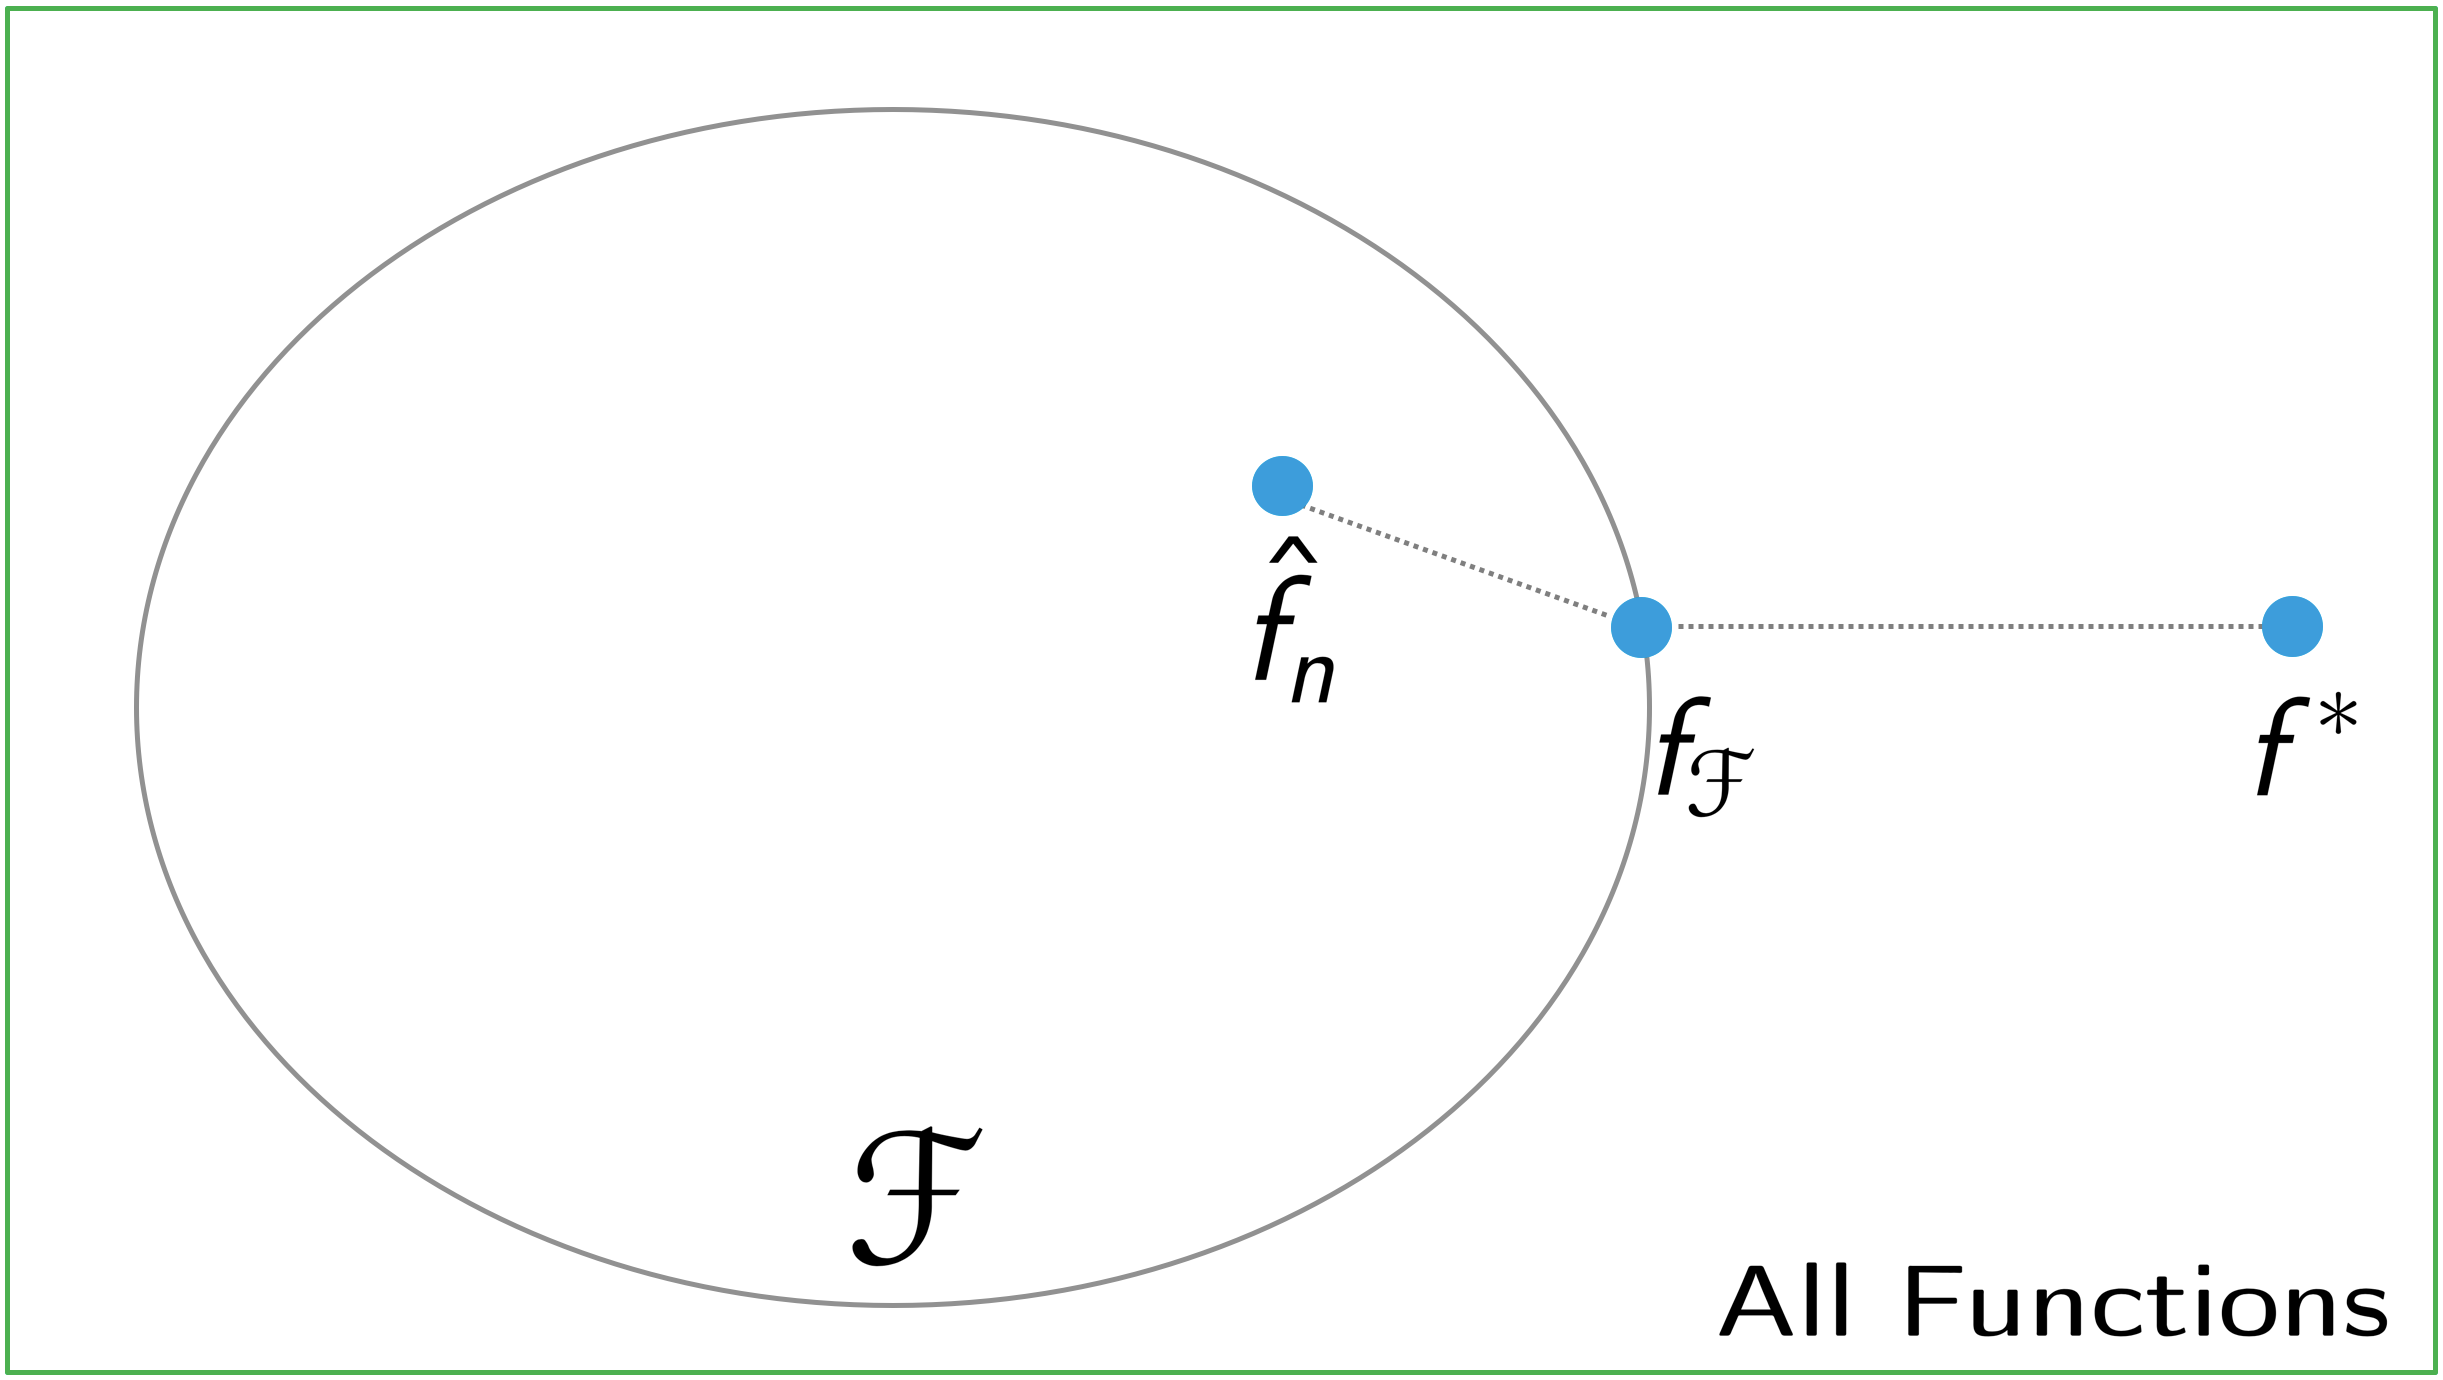
\includegraphics[width=1\columnwidth]{../Figures/ApproxEstError/est-approx}

\column{.4\textwidth}

\begin{align*}
f^{*}= & \argmin_{f}\ex\ell(f(X),Y)\\
f_{\cf}= & \argmin_{f\in\cf}\ex\ell(f(X),Y))\\
\hat{f}_{n}= & \argmin_{f\in\cf}\frac{1}{n}\sum_{i=1}^{n}\ell(f(x_{i}),y_{i})
\end{align*}
\\

\end{columns}


\pause{}
\end{block}
\begin{itemize}
\item \textbf{Approximation Error }(of $\cf$)\textbf{ $=\ R(f_{\cf})-R(\minimizer f)$}
\end{itemize}

\pause{}
\begin{itemize}
\item \textbf{Estimation error} (of $\hat{f}_{n}$ in $\cf$) $=\ R(\hat{f}_{n})-R(f_{\cf})$ 
\end{itemize}
\end{frame}
%
\begin{frame}{Excess Risk Decomposition for ERM}
\begin{itemize}
\item The excess risk of the ERM $\hat{f}_{n}$ can be decomposed:
\begin{eqnarray*}
\mbox{\textbf{Excess Risk}}(\hat{f}_{n}) & = & \risk(\hat{f}_{n})-\risk(\minimizer f)\\
\pause & = & \underbrace{\risk(\hat{f}_{n})-\risk(f_{\cf})}_{\text{estimation error}}+\underbrace{\risk(f_{\cf})-\risk(\minimizer f)}_{\text{approximation error}}.
\end{eqnarray*}
\end{itemize}
\end{frame}
%
\begin{frame}{Optimization Error}
\begin{itemize}
\item In practice, we don't find the ERM $\hat{f}_{n}\in\cf$. 
\item Optimization algorithm returns $\tilde{f}_{n}\in\cf$ , which we hope
is good enough.

\pause{}
\item \textbf{Optimization error: }If $\tilde{f}_{n}$ is the function our
optimization method returns, and $\hat{f}_{n}$ is the empirical risk
minimizer, then
\[
\mbox{Optimization Error }=\;R(\tilde{f}_{n})-R(\hat{f}_{n}).
\]
 

\pause{}
\item Extended decomposition:
\begin{align*}
\mbox{\textbf{Excess Risk}}(\tilde{f}_{n})\, & =\,\risk(\tilde{f}_{n})-\risk(\minimizer f)\\
 & =\underbrace{\risk(\tilde{f}_{n})-R(\hat{f}_{n})}_{\text{optimization error}}+\underbrace{\risk(\hat{f}_{n})-\risk(f_{\cf})}_{\text{estimation error}}+\underbrace{\risk(f_{\cf})-\risk(\minimizer f)}_{\text{approximation error}}
\end{align*}
\end{itemize}


\end{frame}
%

\begin{frame}{Question}
Select true of false for each of the following statements:
\begin{enumerate}
\item Approximation Error is a Random Variable
\item Estimation Error is a Random Variable
\item Optimization Error is a Random Variable. 
\item If the hypothesis space consists of all possible functions functions, then approximation error is non-zero. 
\item Estimation Error can be negative. 
\item Optimization Error can be negative.
\item  The empirical risk of the ERM, $\hat{R}(\hat{f} )$, is an unbiased estimator of the risk of the ERM $R(\hat{f} )$. Does your answer change if it's a $\hat{R}(f)$ where $f$ is independent of training data?
\end{enumerate}
\end{frame}

\begin{frame}{Question}
For each, use $\leq$, $\geq$, or $=$ to determine the
  relationship between the two quantities,
  or if the relationship cannot be determined.
  Throughout assume $\mathcal{F}_1,\mathcal{F}_2$ are hypothesis spaces with
  $\mathcal{F}_1 \subset \mathcal{F}_2$, and assume we are working with a fixed loss
  function $\ell$.
  \begin{enumerate}
  \item The estimation errors of two decision functions $f_1,f_2$ that
    minimize the empirical risk over the same hypothesis space,
    where $f_2$ uses 5 extra data points.
  \item The approximation errors of the two decision functions
    $f_1,f_2$ that minimize risk with respect to $\mathcal{F}_1,\mathcal{F}_2$,
    respectively (i.e., $f_1=f_{\mathcal{F}_1}$ and $f_2=f_{\mathcal{F}_2}$).
  \item The empirical risks of two decision functions $f_1,f_2$ that
    minimize the empirical risk over $\mathcal{F}_1,\mathcal{F}_2$, respectively.
    Both use the same fixed training data.
  \item The estimation errors (for $\mathcal{F}_1,\mathcal{F}_2$, respectively) of two decision functions $f_1,f_2$ that
    minimize the empirical risk over $\mathcal{F}_1,\mathcal{F}_2$, respectively.
  \item The risk of two decision functions $f_1,f_2$ that
    minimize the empirical risk over $\mathcal{F}_1,\mathcal{F}_2$, respectively.
  \end{enumerate}
\end{frame}

\begin{frame}{Solution}
\begin{enumerate}
  \item Roughly speaking, more data is better, so we would tend to expect
    that $f_2$ will have lower estimation error.  That said, this is
    not always the case, so the relationship cannot be determined.
  \item The approximation error of $f_1$ will be larger.
  \item The empirical risk of $f_1$ will be larger.
  \item Roughly speaking, increasing the hypothesis space should
    increase the estimation error since the approximation error will
    decrease, and we expect to need more data.  That said, this
    is not always the case, so the answer is the relationship cannot
    be determined.
  \item Cannot be determined.
  \end{enumerate}
\end{frame}

\section{Regularization}

\begin{frame}{Constrained Empirical Risk Minimization}
\begin{block}{Constrained ERM (Ivanov regularization)}

For complexity measure $\Omega:\cf\to[0,\infty)$ and fixed $r\ge0$,

\begin{align*}
\min_{f\in\cf}\; & \frac{1}{n}\sum_{i=1}^{n}\ell(f(x_{i}),y_{i})\\
\mbox{s.t.}\; & \Omega(f)\le r
\end{align*}


\pause{}
\end{block}
\begin{itemize}
\item Choose $r$ using validation data or cross-validation.

\pause{}
\item Each $r$ corresponds to a different hypothesis spaces. Could also
write:
\[
\min_{f\in\cf_{r}}\frac{1}{n}\sum_{i=1}^{n}\ell(f(x_{i}),y_{i})
\]
\end{itemize}
\end{frame}
%
\begin{frame}{Penalized Empirical Risk Minimization}
\begin{block}{Penalized ERM (Tikhonov regularization)}

For complexity measure $\Omega:\cf\to[0,\infty)$ and fixed $\lambda\ge0$,
\begin{align*}
\min_{f\in\cf} & \frac{1}{n}\sum_{i=1}^{n}\ell(f(x_{i}),y_{i})+\lambda\Omega(f)
\end{align*}

\end{block}
\begin{itemize}
\item Choose $\lambda$ using validation data or cross-validation.

\pause{}
\item (Ridge regression in homework is of this form.)
\end{itemize}
\end{frame}
%
\begin{frame}{Ridge Regression: Workhorse of Modern Data Science}
\begin{block}{Ridge Regression (Tikhonov Form)}

The ridge regression solution for regularization parameter $\lambda\ge0$
is
\[
\hat{w}=\argmin_{w\in\reals^{d}}\frac{1}{n}\sum_{i=1}^{n}\left\{ w^{T}x_{i}-y_{i}\right\} ^{2}+\lambda\|w\|_{2}^{2},
\]
where $\|w\|_{2}^{2}=w_{1}^{2}+\cdots+w_{d}^{2}$ is the square of
the $\ell_{2}$-norm.

\pause{}

\end{block}

\begin{block}{Ridge Regression (Ivanov Form)}
 

The ridge regression solution for complexity parameter $r\ge0$ is
\[
\hat{w}=\argmin_{\|w\|_{2}^{2}\le r^{2}}\frac{1}{n}\sum_{i=1}^{n}\left\{ w^{T}x_{i}-y_{i}\right\} ^{2}.
\]

\end{block}
\end{frame}
%
\begin{frame}{Lasso Regression: Workhorse (2) of Modern Data Science}
\begin{block}{Lasso Regression (Tikhonov Form)}

The lasso regression solution for regularization parameter $\lambda\ge0$
is
\[
\hat{w}=\argmin_{w\in\reals^{d}}\frac{1}{n}\sum_{i=1}^{n}\left\{ w^{T}x_{i}-y_{i}\right\} ^{2}+\lambda\|w\|_{1},
\]
where $\|w\|_{1}=\left|w_{1}\right|+\cdots+\left|w_{d}\right|$ is
the $\ell_{1}$-norm.

\pause{}

\end{block}

\begin{block}{Lasso Regression (Ivanov Form)}
 

The lasso regression solution for complexity parameter $r\ge0$ is
\[
\hat{w}=\argmin_{\|w\|_{1}\le r}\frac{1}{n}\sum_{i=1}^{n}\left\{ w^{T}x_{i}-y_{i}\right\} ^{2}.
\]

\end{block}
\end{frame}
%
\begin{frame}{Ridge vs. Lasso: Regularization Paths}

\let\thefootnote\relax\footnotetext{\tiny{Modified from Hastie, Tibshirani, and Wainwright's \emph{Statistical Learning with Sparsity}, Fig 2.1. About predicting crime in 50 US cities.}}
\begin{center}
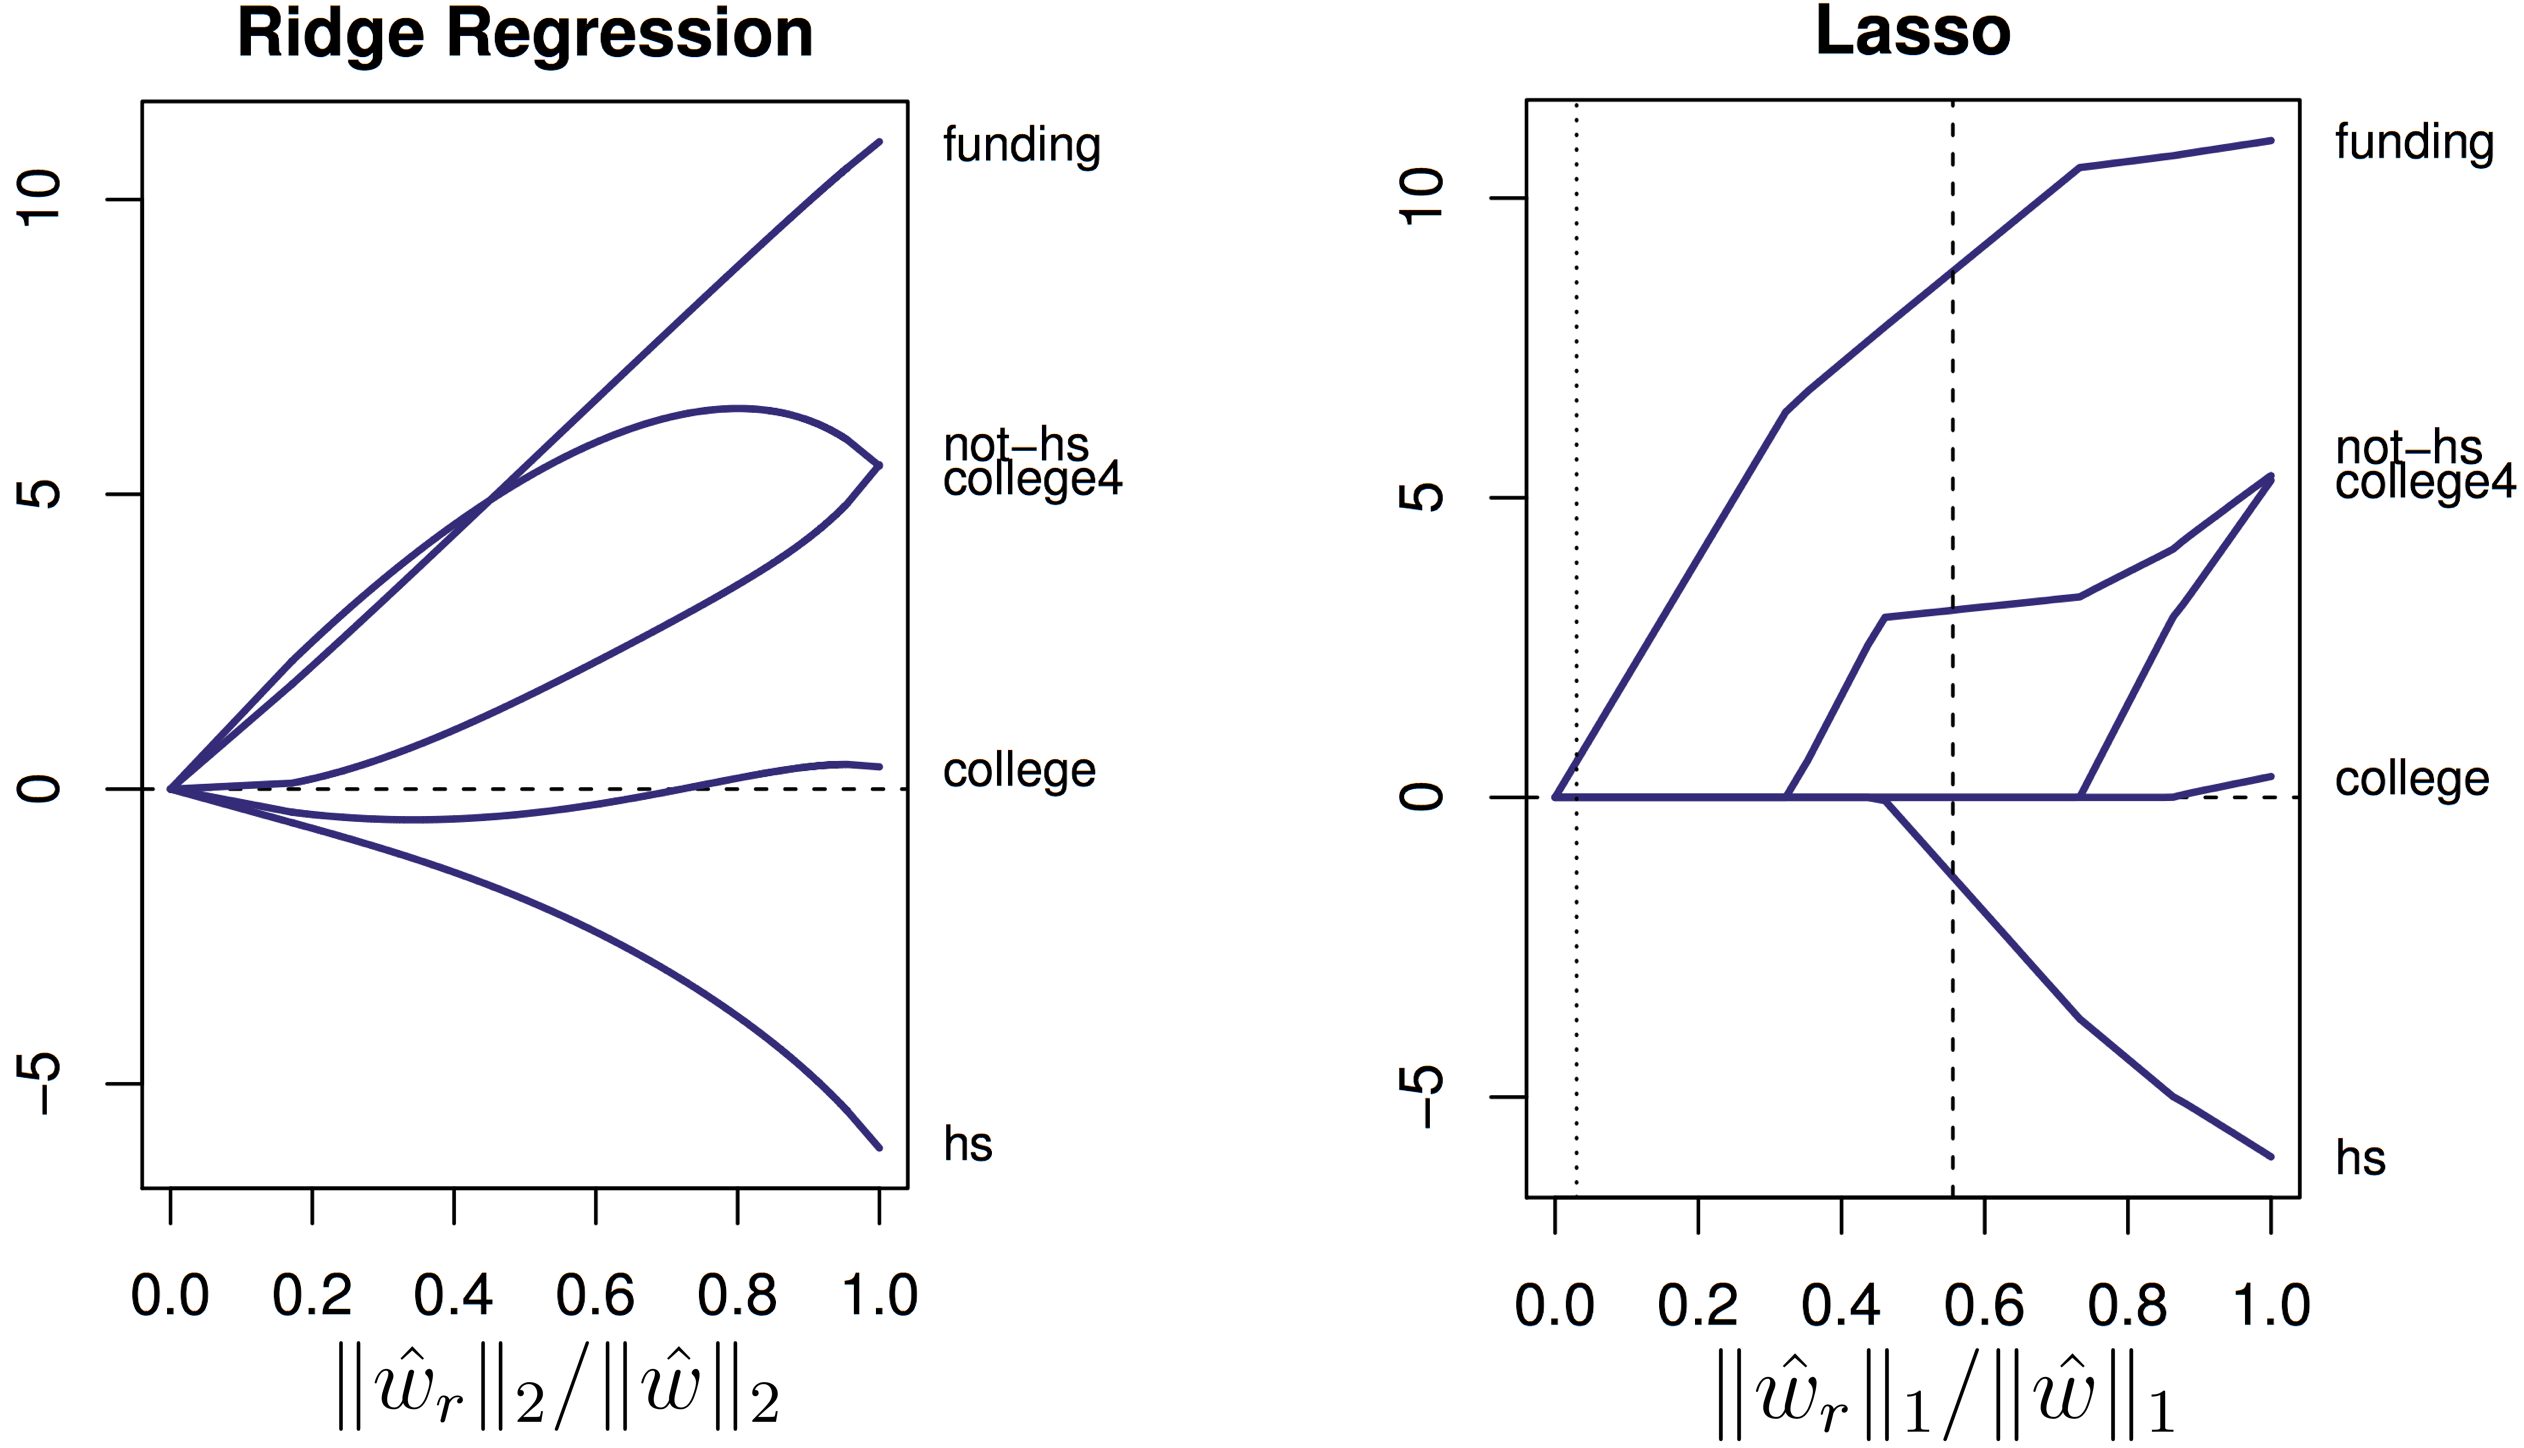
\includegraphics[height=0.8\textheight]{../Figures/L1L2/lasso-ridge-paths-side-by-side}
\par\end{center}

\end{frame}
%
\begin{frame}{Linearly Dependent Features: Take Away}
\begin{itemize}
\item For identical features
\begin{itemize}
\item $\ell_{1}$ regularization spreads weight arbitrarily (all weights
same sign)
\item $\ell_{2}$ regularization spreads weight evenly 
\end{itemize}
\item Linearly related features
\begin{itemize}
\item $\ell_{1}$ regularization chooses variable with larger scale, 0 weight
to others
\item $\ell_{2}$ prefers variables with larger scale -- spreads weight
proportional to scale
\end{itemize}
\end{itemize}
\end{frame}
%
\begin{frame}{Correlated Features, $\ell_{1}$ Regularization}
\begin{center}
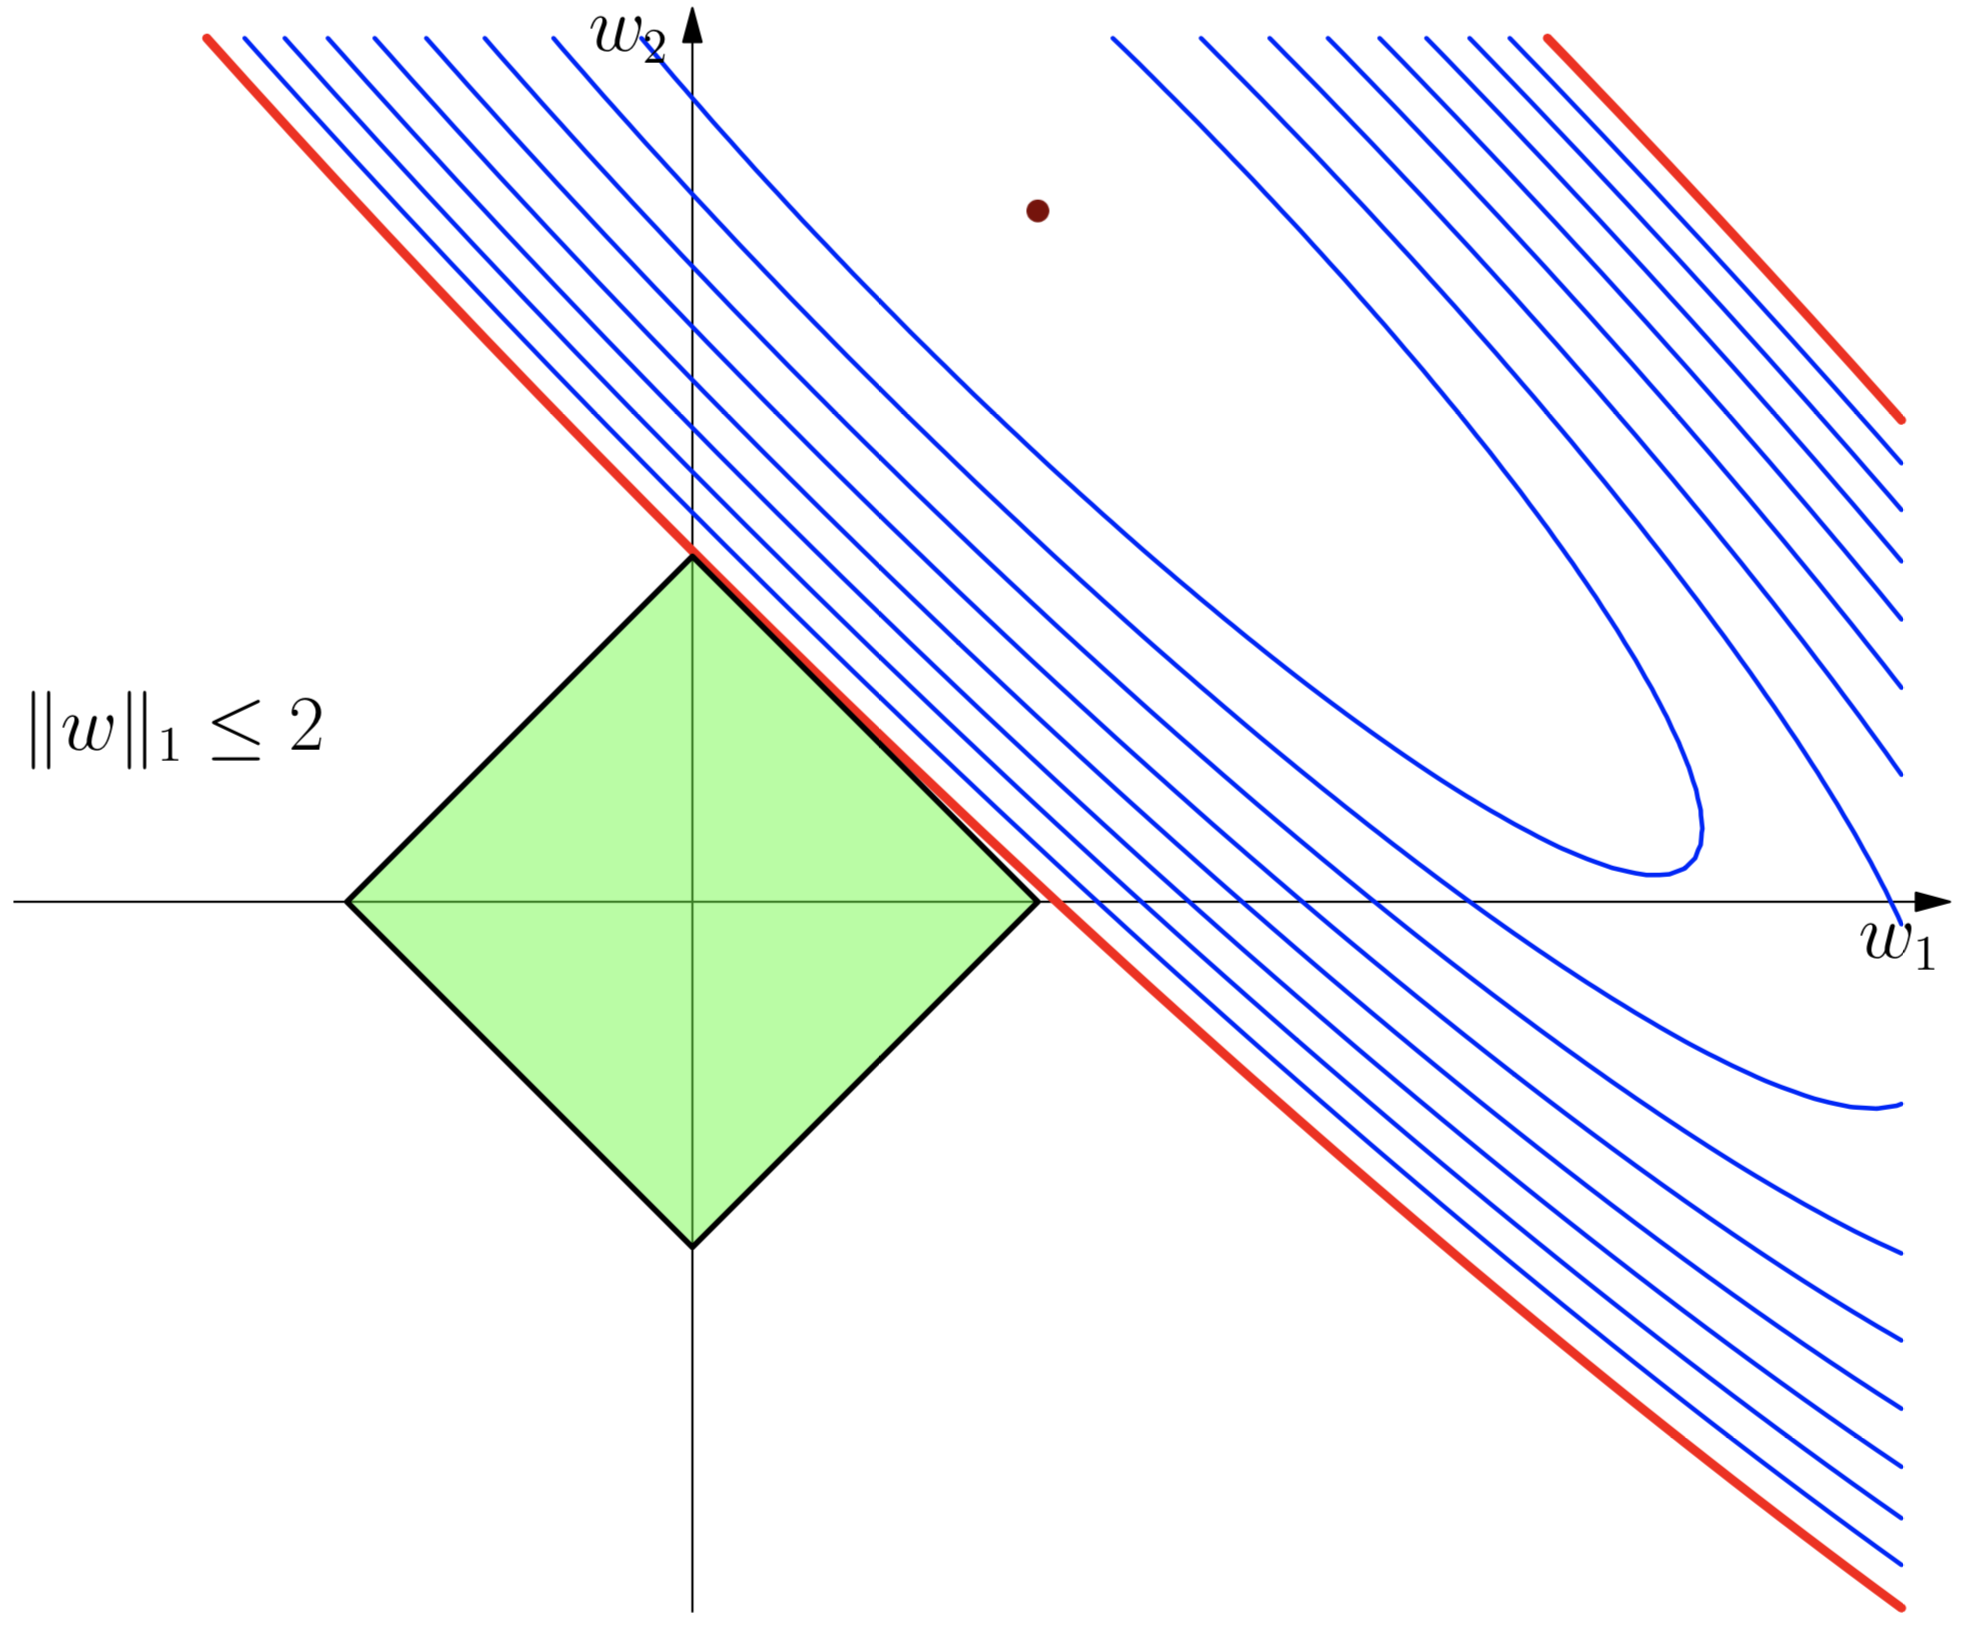
\includegraphics[height=0.4\textheight]{../Figures/L1L2/L1Corr}\hspace{0.2\textwidth}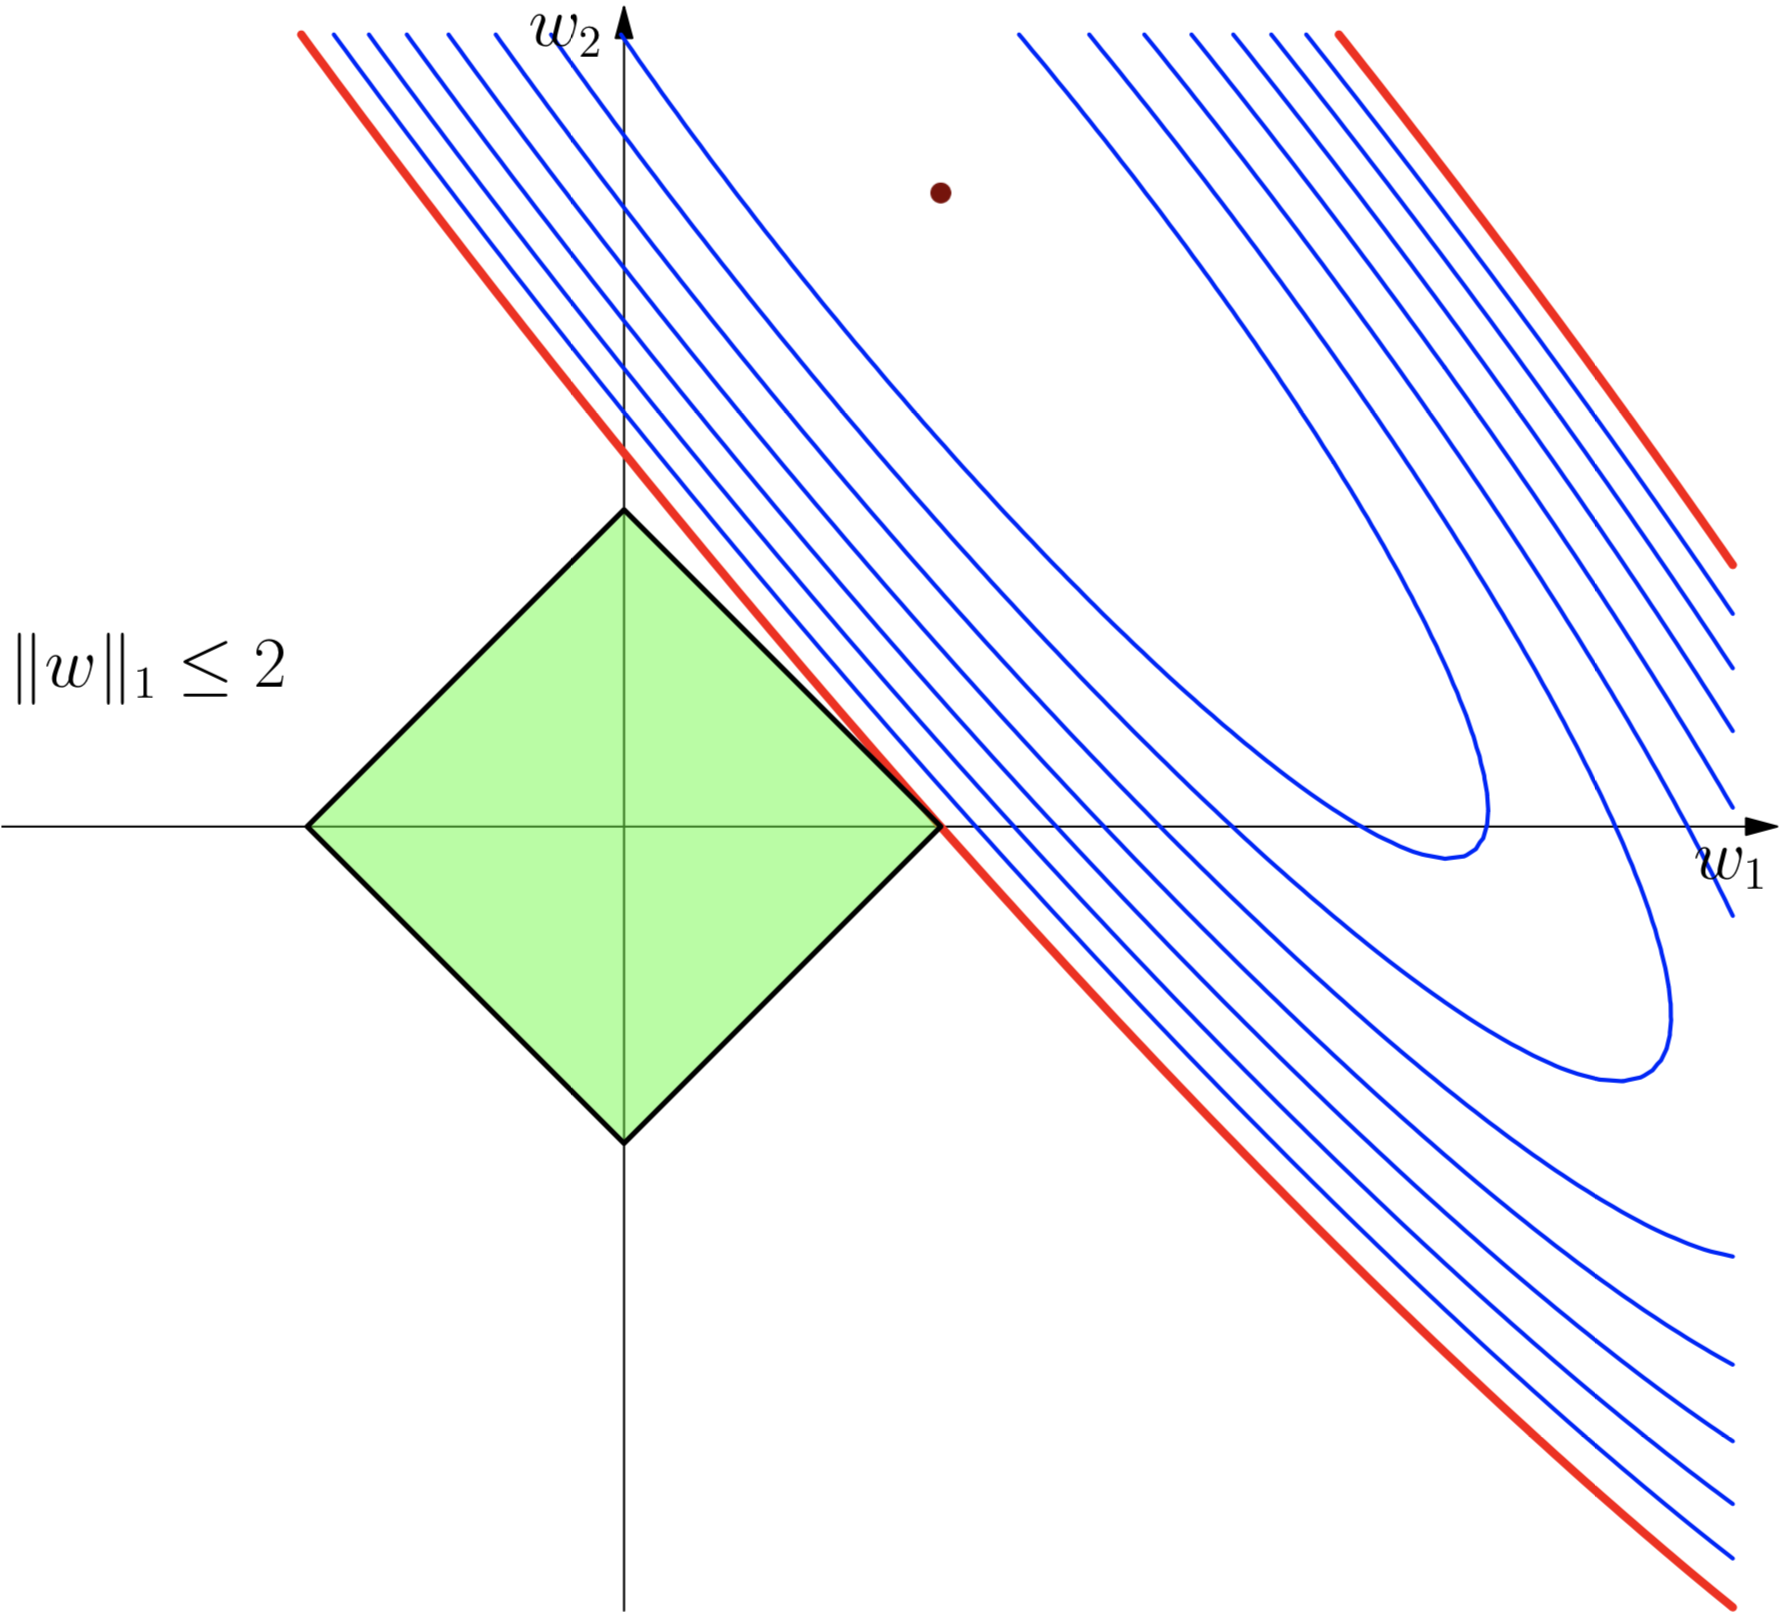
\includegraphics[height=0.4\textheight]{../Figures/L1L2/L1Corr2}
\par\end{center}
\begin{itemize}
\item Intersection could be anywhere on the top right edge. 
\item Minor perturbations (in data) can drastically change intersection
point -- very unstable solution.
\item Makes division of weight among highly correlated features (of same
scale) seem arbitrary.
\begin{itemize}
\item If $x_{1}\approx2x_{2}$, ellipse changes orientation and we hit a
corner. (Which one?)
\end{itemize}
\end{itemize}
\end{frame}
%
\begin{frame}{Elastic Net}
\begin{itemize}
\item The \textbf{elastic net} combines lasso and ridge penalties:
\[
\hat{w}=\argmin_{w\in\reals^{d}}\frac{1}{n}\sum_{i=1}^{n}\left\{ w^{T}x_{i}-y_{i}\right\} ^{2}+\lambda_{1}\|w\|_{1}+\lambda_{2}\|w\|_{2}^{2}
\]
\end{itemize}

\pause{}
\begin{itemize}
\item We expect correlated random variables to have similar coefficients.
\end{itemize}
\end{frame}
%
\begin{frame}{Highly Correlated Features, Elastic Net Constraint}
\begin{center}
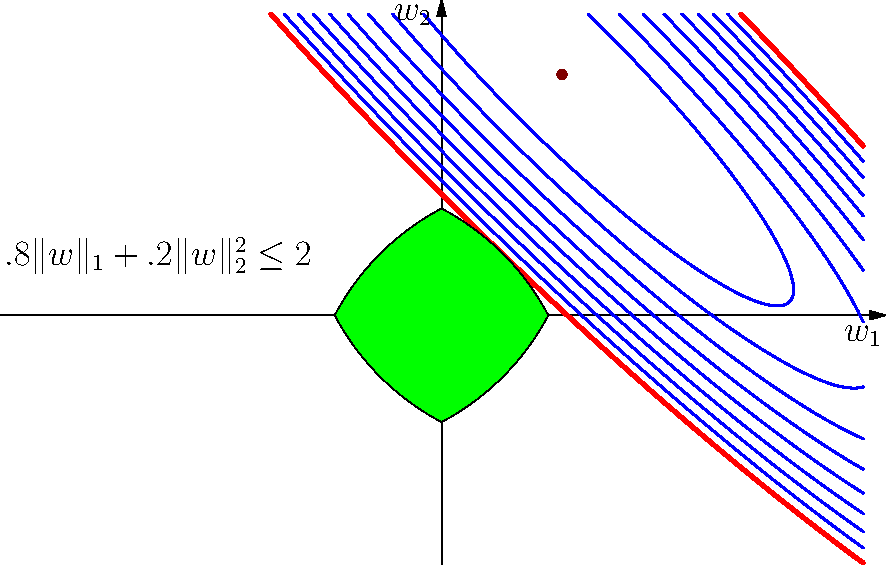
\includegraphics[height=0.5\textheight]{../Figures/L1L2/EnetCorr}
\par\end{center}
\begin{itemize}
\item Elastic net solution is closer to $w_{2}=w_{1}$ line, despite high
correlation.
\end{itemize}
\end{frame}
%
\begin{frame}{Elastic Net Results on Model}
\begin{center}
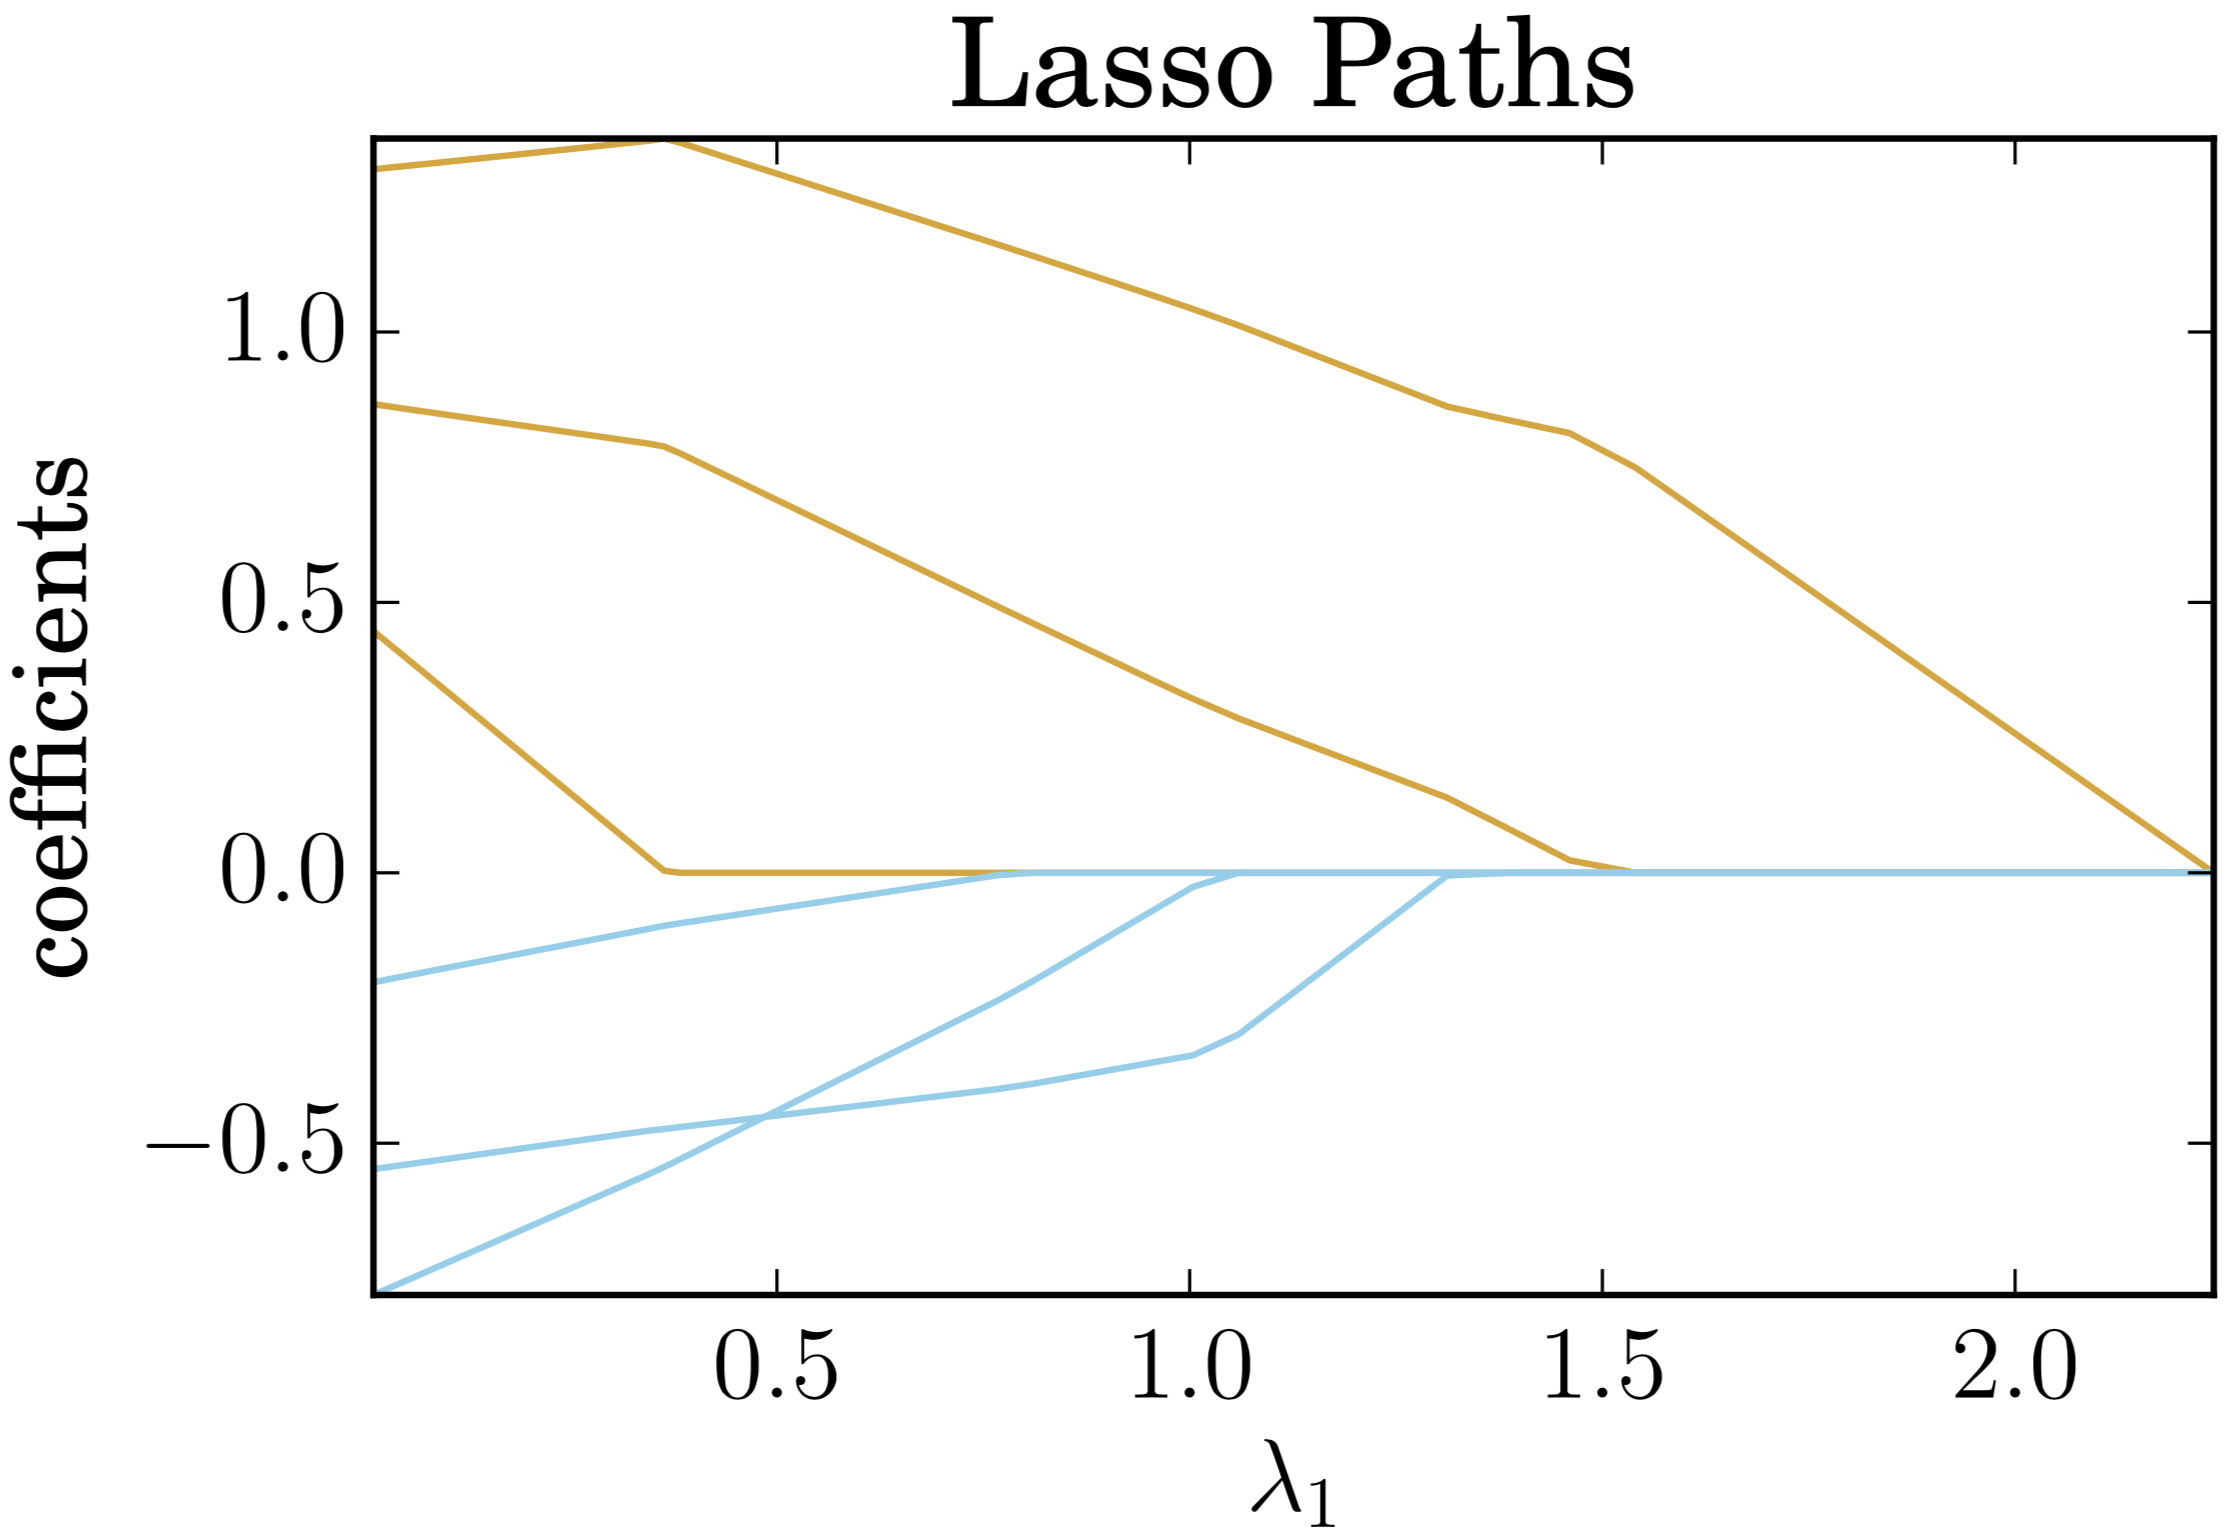
\includegraphics[height=0.6\textheight]{../Figures/L1L2/L1regpaths-correlated-vars}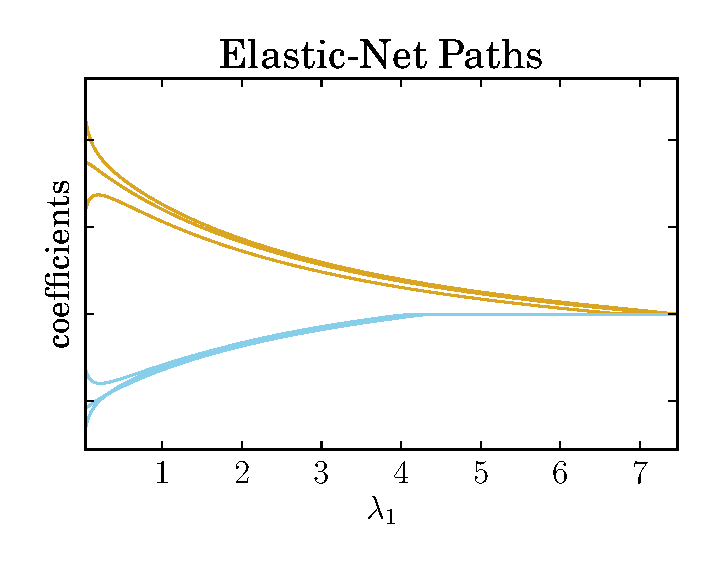
\includegraphics[height=0.6\textheight]{../Figures/L1L2/elasticNetregpaths-correlated-vars}
\par\end{center}
\begin{itemize}
\item Lasso on left; Elastic net on right.
\item Ratio of $\ell_{2}$ to $\ell_{1}$ regularization roughly $2:1$.
\end{itemize}
\end{frame}
%
%\begin{frame}{Elastic Net - ``Sparse Regions''}
%
%\let\thefootnote\relax\footnotetext{\tiny{Fig from \href{https://arxiv.org/abs/1411.3230}{Mairal et al.'s Sparse Modeling for Image and Vision Processing} Fig 1.9}}
%\begin{center}
%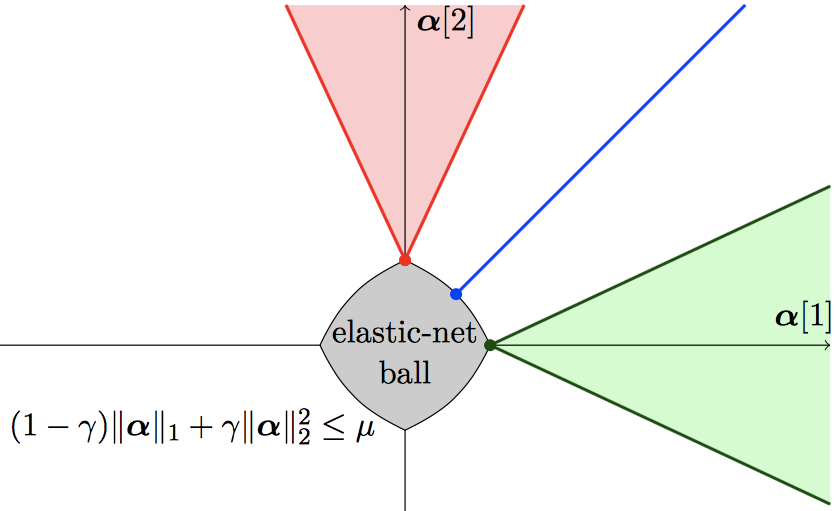
\includegraphics[height=0.5\textheight]{../Figures/L1L2/projections-to-ElasticNetBall}\vspace{-0.3cm}
%\par\end{center}
%\begin{itemize}
%\item Suppose design matrix $X$ is orthogonal, so $X^{T}X=I$, and contours
%are circles (and features uncorrelated)
%\item Then OLS solution in green or red regions implies elastic-net constrained
%solution will be at corner
%\end{itemize}
%\end{frame}
%
\begin{frame}{Elastic Net Summary}
\begin{itemize}
\item With uncorrelated features, we can get sparsity.
\item Among correlated features (same scale), we spread weight more evenly. 
\end{itemize}
\end{frame}
%
\begin{frame}{Question on correlated features}
We solve lasso and ridge regression where input lives in $\mathcal{R}^4$. The first two features of all the input vector are duplicates of each other, or $x_{i1} = x_{i2}$ for all $i$. Consider the following weight vectors:
\begin{enumerate}
\item $(0, 1.2, 6.7, 2.1)^T$
\item $(0.6, 0.6,  6.7, 2.1)^T$
\item $(1.2, 0, 6.7, 2.1)^T$
\item $(-0.1, 1.3 , 6.7, 2.1)^T$
\end{enumerate}

Which of them are valid solution for a) Ridge Regression and b) Lasso Regression?
\end{frame}
%
\begin{frame}{Finding Lasso Solution}
\begin{itemize}
\item Many options.

\pause{}
\item Convert to quadratic program using positive/negative parts
\begin{align*}
\min_{w^{+},w^{-}}\quad & \sum_{i=1}^{n}\left(\left(w^{+}-w^{-}\right)^{T}x_{i}-y_{i}\right)^{2}+\lambda1^{T}\left(w^{+}+w^{-}\right)\\
\mbox{subject to}\quad & w_{i}^{+}\ge0\mbox{ for all }i\text{\qquad}w_{i}^{-}\ge0\mbox{ for all }i,
\end{align*}


\pause{}
\item Coordinate descent

\pause{}
\begin{itemize}
\item Lasso has closed form solution for coordinate minimizers!

\pause{}
\end{itemize}
\item Subgradient descent
\end{itemize}
\end{frame}

\section{Optimization}
\begin{frame}{Gradient Descent for Empirical Risk and Averages}
\begin{itemize}
\item Suppose we have a hypothesis space of functions $\cf=\left\{ f_{w}:\cx\to\ca\mid w\in\reals^{d}\right\} $ 
\begin{itemize}
\item Parameterized by $w\in\reals^{d}$.
\end{itemize}

\pause{}
\item ERM is to find $w$ minimizing
\[
\hat{R}_{n}(w)=\frac{1}{n}\sum_{i=1}^{n}\loss(f_{w}(x_{i}),y_{i})
\]
\end{itemize}

\pause{}
\begin{itemize}
\item Suppose $\loss(f_{w}(x_{i}),y_{i})$ is differentiable as a function
of $w$.
\end{itemize}

\pause{}
\begin{itemize}
\item Then we can do gradient descent on $\hat{R}_{n}(w)$...
\end{itemize}
\end{frame}

\begin{frame}{Gradient Descent: How does it scale with $n$?}
\begin{itemize}
\item At every iteration, we compute the gradient at current $w$:
\[
\del\hat{R}_{n}(w)=\frac{1}{n}\sum_{i=1}^{n}\del_{w}\ell(f_{w}(x_{i}),y_{i})
\]
\end{itemize}

\pause{}
\begin{itemize}
\item We have to touch all $n$ training points to take a single step. {[}$O(n)${]}
\end{itemize}

\pause{}
\begin{itemize}
\item What if we just use an estimate of the gradient?
\end{itemize}
\end{frame}
%
\begin{frame}{Minibatch Gradient}
\begin{itemize}
\item The \textbf{full gradient} is
\[
\del\hat{R}_{n}(w)=\frac{1}{n}\sum_{i=1}^{n}\del_{w}\ell(f_{w}(x_{i}),y_{i})
\]
\item It's an average over the \textbf{full batch} of data $\cd_{n}=\left\{ (x_{1},y_{1}),\ldots,(x_{n},y_{n})\right\} $.
\end{itemize}

\pause{}
\begin{itemize}
\item Let's take a random subsample of size $N$ (called a \textbf{minibatch}):
\[
(x_{m_{1}},y_{m_{1}}),\ldots,(x_{m_{N}},y_{m_{N}})
\]
\end{itemize}

\pause{}
\begin{itemize}
\item The \textbf{minibatch gradient is
\[
\del\hat{R}_{N}(w)=\frac{1}{N}\sum_{i=1}^{N}\del_{w}\ell(f_{w}(x_{m_{i}}),y_{m_{i}})
\]
}
\end{itemize}

\pause{}
\begin{itemize}
\item Minibatch gradient is an unbiased estimate of full-batch gradient:
$\ex\left[\del\hat{R}_{N}(w)\right]=\del\hat{R}_{n}(w)$
\end{itemize}
\end{frame}
%
\begin{frame}{How big should minibatch be?}
\begin{itemize}
\item Tradeoffs of minibatch size:
\begin{itemize}
\item Bigger $N$ $\implies$Better estimate of gradient, but slower (more
data to touch)
\item Smaller $N$ $\implies$Worse estimate of gradient, but can be quite
fast 
\end{itemize}
\end{itemize}

\pause{}
\begin{itemize}
\item Even $N=1$ works, it's traditionally called \textbf{stochastic gradient
descent} (SGD).
\end{itemize}

\pause{}
\begin{itemize}
\item Quality of minibatch estimate depends on
\begin{itemize}
\item size of minibatch
\item but is \textbf{independent }of full dataset size $n$
\end{itemize}

\pause{}
\item Discussed in Concept Check question.
\end{itemize}
\end{frame}
%

\begin{frame}{Subgradient Review}
\begin{definition}
[Subgradient and Subdifferential] A vector $g$ is a subgradient of (convex) $f:\mathcal{R}^d \rightarrow \mathcal{R}$ at $x$ if for all $z$ $$f(z) \geq f(x) + g^T(z-x)$$. The set of all subgradients at $x$ is called the subdifferential of $f$ at $x$ $\partial f(x)$
\end{definition}

Questions: 
\begin{enumerate}
\item (True/False) If $f$ is convex and differentiable everywhere in the domain, then $\partial f(x) = \{ \nabla f(x) \}$
\item (True/False) The subdifferential of $f$ at $x$, $\partial f(x)$ is always a convex set. (Null set is trivially complex)
\end{enumerate}
\end{frame}
\begin{frame}{Descent Directions}
\begin{itemize}
\item A step direction is a \textbf{descent direction} if, for small enough
step size, the objective function value always decreases.
\end{itemize}

\pause{}
\begin{itemize}
\item Negative gradient is a descent direction.
\end{itemize}

\pause{}
\begin{itemize}
\item A negative subgradient is \textbf{not} a descent direction. But always
\textbf{takes you closer to a minimizer}.

\pause{}
\item Negative stochastic or minibatch gradient direction is \textbf{not}
a descent direction. But we have convergence theorems.

\pause{}
\item Negative stochastic subgradient step direction is \textbf{not} a descent
direction. But we have convergence theorems (not discussed in class).
\end{itemize}
\end{frame}

\section{Classification}
\begin{frame}{The Score Function}
\begin{itemize}
\item Action space $\ca=\reals\qquad$ Output space $\cy=\left\{ -1,1\right\} $
\item \textbf{Real-valued prediction function} $f:\cx\to\reals$

\pause{}

\end{itemize}
\begin{definition}
The value $f(x)$ is called the \textbf{score} for the input $x$. 
\end{definition}

\begin{itemize}
\item In this context, $f$ may be called a \textbf{score function}.

\pause{}
\item Intuitively, magnitude of the score represents the \textbf{confidence
of our prediction}.
\end{itemize}
\end{frame}
%
\begin{frame}{The Margin}
\begin{definition}
The \textbf{margin} (or \textbf{functional margin})\textbf{ }for predicted
score $\hat{y}$ and true class $y\in\left\{ -1,1\right\} $ is $y\hat{y}$. 
\end{definition}


\pause{}
\begin{itemize}
\item The margin often looks like $yf(x)$, where $f(x)$ is our score function.

\pause{}
\item The margin is a measure of how \textbf{correct} we are.

\pause{}
\begin{itemize}
\item If $y$ and $\hat{y}$ are the same sign, prediction is \textbf{correct}
and margin is \textbf{positive}.
\item If $y$ and $\hat{y}$ have different sign, prediction is \textbf{incorrect}
and margin is \textbf{negative}.
\end{itemize}
\end{itemize}

\pause{}
\begin{itemize}
\item We want to \textbf{maximize the margin}.
\end{itemize}
\end{frame}
%
\begin{frame}{Classification Losses}

Logistic/Log loss: $\loss_{\text{Logistic}}=\log\left(1+e^{-m}\right)$
\begin{center}
\includegraphics[height=0.7\textheight]{../Figures/loss-functions/loss\lyxdot Zero_One\lyxdot Hinge\lyxdot Logistic}
\par\end{center}

Logistic loss is differentiable. Logistic loss always wants more margin
(loss never 0).
\end{frame}
%
\begin{frame}{Support Vector Machine }
\begin{itemize}
\item Hypothesis space $\cf=\left\{ f(x)=w^{T}x+b\mid w\in\reals^{d},\,b\in\reals\right\} $.
\end{itemize}

\pause{}
\begin{itemize}
\item $\ell_{2}$ regularization (Tikhonov style)
\item Loss $\ell(m)=\max\left\{ 1-m,0\right\} $
\end{itemize}

\pause{}
\begin{itemize}
\item The SVM prediction function is the solution to
\[
\min_{w\in\reals^{d},b\in\reals}\frac{1}{2}||w||^{2}+\frac{c}{n}\sum_{i=1}^{n}\max\left(0,1-y_{i}\left[w^{T}x_{i}+b\right]\right).
\]
 
\end{itemize}
\end{frame}
%
\begin{frame}{SVM as a Quadratic Program}
\begin{itemize}
\item The SVM optimization problem is equivalent to
\begin{eqnarray*}
\textrm{minimize} &  & \frac{1}{2}||w||^{2}+\frac{c}{n}\sum_{i=1}^{n}\xi_{i}\\
\textrm{subject to} &  & -\xi_{i}\le0\;\mbox{for }i=1,\ldots,n\\
 &  & \left(1-y_{i}\left[w^{T}x_{i}+b\right]\right)-\xi_{i}\le0\;\mbox{for }i=1,\ldots,n
\end{eqnarray*}


\pause{}
\item Differentiable objective function
\item $n+d+1$ unknowns and $2n$ affine constraints. 

\pause{}
\item A quadratic program that can be solved by any off-the-shelf QP solver. 

\item We arrived at this optimization problem also from a geometric prospective.
\end{itemize}
\end{frame}
%

\begin{frame}{Linear Separability and Hard Margin SVM}
\begin{definition}
[Linear Separability] We say $(x_i,y_i)$ for $i=1,\ldots,n$ are \textit{linearly separable} if there is a $w\in \mathcal{R}^d$ and $b\in \mathcal{R}$ such that $y_i(w^Tx_i-b)>0$ for all $i$. The set $\{v\in \mathcal{R}^d\mid w^Tv-b=0\}$ is called a \textit{separating hyperplane}.
\end{definition}


%For Hard Margin SVM we solve the following optimization problem:
%$$\begin{array}{ll}
%  \text{minimize}_{w,b} & \|w\|_2^2\\
%  \text{subject to} & y_i(w^Tx_i-b) \geq 1\quad\text{for all $i$.}
%\end{array}$$
\end{frame}

\begin{frame}{Maximum Margin Separating Hyperplane}
\begin{center}
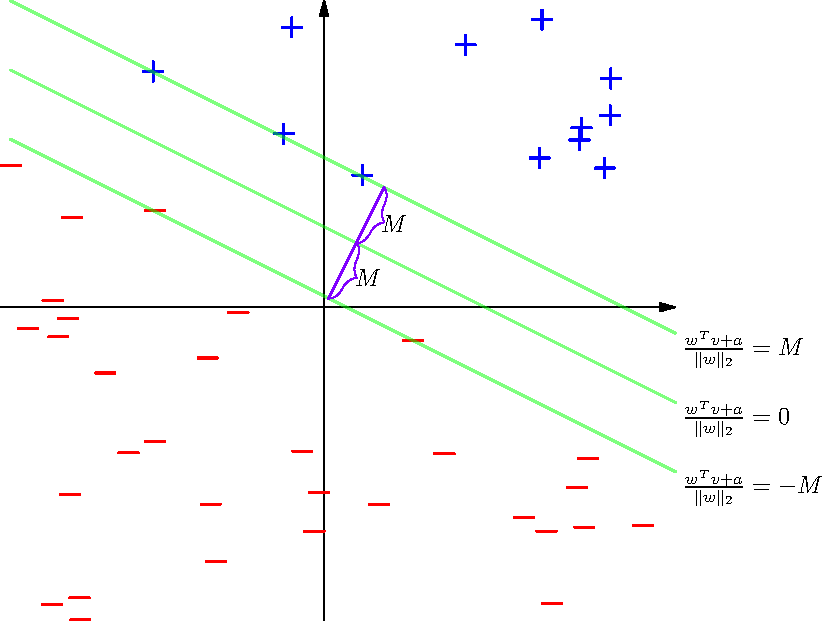
\includegraphics[height=0.8\textheight]{3-SVM/MaxMargin.pdf}
\par\end{center}
\end{frame}


\begin{frame}[fragile]
  \frametitle{Soft Margin SVM (unlabeled points have $\xi_i=0$)}
\begin{center}
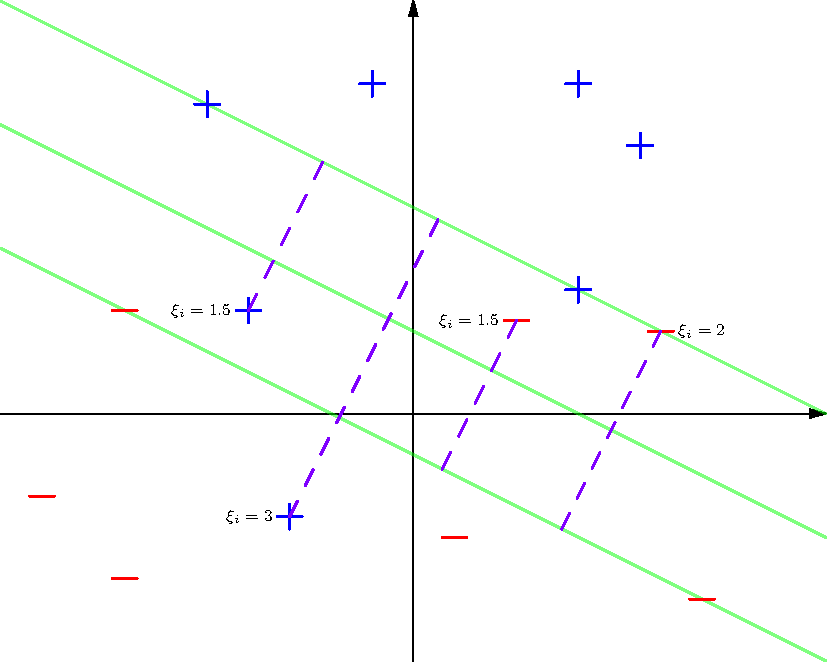
\includegraphics[height=0.8\textheight]{3-SVM/SoftMargin.pdf}
\par\end{center}
\end{frame}

\section{The Representer Theorem and Kernelization}
\begin{frame}{General Objective Function for Linear Hypothesis Space (Details)}
\begin{itemize}
\item \textbf{Generalized objective}: 
\[
\min_{w\in\ch}R\left(\|w\|\right)+L\left(\left\langle w,x_{1}\right\rangle ,\ldots,\left\langle w,x_{n}\right\rangle \right),
\]
where
\begin{itemize}
\item $w,x_{1},\ldots,x_{n}\in\ch$ for some Hilbert space $\ch$. (We typically
have $\ch=\reals^{d}.)$
\item $\|\cdot\|$ is the norm corresponding to the inner product of $\ch$.
(i.e. $\|w\|=\sqrt{\left\langle w,w\right\rangle }$) 
\item $R:[0,\infty)\to\reals$ is nondecreasing (\textbf{Regularization
term}), and
\item $L:\reals^{n}\to\reals$ is arbitrary (\textbf{Loss term}).
\end{itemize}
\end{itemize}

\pause{}
\begin{itemize}
\item Ridge regression and SVM are of this form. 

\pause{}
\item What if we use lasso regression? $\pause$No! $\ell_{1}$ norm does
not correspond to an inner product. 
\end{itemize}
\end{frame}
%
\begin{frame}{The Representer Theorem}

Let $J(w)=R\left(\|w\|\right)+L\left(\left\langle w,x_{1}\right\rangle ,\ldots,\left\langle w,x_{n}\right\rangle \right)$
under conditions described above.
\begin{theorem}
[Representer Theorem]If $J(w)$ has a minimizer, then it \textbf{has
a minimizer of the form} 
\[
w^{*}=\sum_{i=1}^{n}\alpha_{i}x_{i}.
\]
If $R$ is strictly increasing, then all minimizers have this form.
\end{theorem}


\pause{}

Basic idea of proof:
\begin{itemize}
\item Let $M=\linspan\left(x_{1},\ldots,x_{n}\right)$. {[}the \textbf{``span
of the data}''{]}
\item Let $w=\proj_{M}w^{*}$, for some minimizer $w^{*}$ of $J(w)$.
\item Then $\left\langle w,x_{i}\right\rangle =\left\langle w^{*},x_{i}\right\rangle $,
so loss part doesn't change.
\item $\|w\|\le\|w^{*}\|$, since projection reduces norm. So regularization
piece never increases.
\end{itemize}
\end{frame}
%
\begin{frame}{Reparametrization with Representer Theorem}
 
\begin{itemize}
\item Original plan: 
\begin{itemize}
\item Find $w^{*}\in\argmin_{w\in\ch}R\left(\|w\|\right)+L\left(\left\langle w,x_{1}\right\rangle ,\ldots,\left\langle w,x_{n}\right\rangle \right)$
\item Predict with $\hat{f}(x)=\left\langle w^{*},x\right\rangle $.
\end{itemize}

\pause{}
\item Plugging in result of representer theorem, it's equivalent to
\begin{itemize}
\item Find $\alpha^{*}\in\argmin_{\alpha\in\reals^{n}}R\left(\sqrt{\alpha^{T}K\alpha}\right)+L\left(K\alpha\right)$
\item Predict with $\hat{f}(x)=k_{x}^{T}\alpha^{*}\pause$, where
\[
K=\begin{pmatrix}\left\langle x_{1},x_{1}\right\rangle  & \cdots & \left\langle x_{1},x_{n}\right\rangle \\
\vdots & \ddots & \cdots\\
\left\langle x_{n},x_{1}\right\rangle  & \cdots & \left\langle x_{n},x_{n}\right\rangle 
\end{pmatrix}\qquad\text{and}\qquad k_{x}=\begin{pmatrix}\left\langle x_{1},x\right\rangle \\
\vdots\\
\left\langle x_{n},x\right\rangle 
\end{pmatrix}
\]
\end{itemize}

\pause{}
\begin{itemize}
\item Every element $x\in\ch$ occurs inside an inner products with a training
input $x_{i}\in\ch$.
\end{itemize}
\end{itemize}
\end{frame}
%
\begin{frame}{Kernelization}

\begin{definition}
A method is \textbf{kernelized }if every feature vector $\psi(x)$
only appears inside an inner product with another feature vector $\psi(x')$.
This applies to both the optimization problem and the prediction function.
\end{definition}


\pause{}
\begin{itemize}
\item Here we are using $\psi(x)=x$. Thus finding 
\[
\alpha^{*}\in\argmin_{\alpha\in\reals^{n}}R\left(\sqrt{\alpha^{T}K\alpha}\right)+L\left(K\alpha\right)
\]
 and making predictions with $\hat{f}(x)=k_{x}^{T}\alpha^{*}$ is
a \textbf{kernelization} of finding
\[
w^{*}\in\argmin_{w\in\ch}R\left(\|w\|\right)+L\left(\left\langle w,x_{1}\right\rangle ,\ldots,\left\langle w,x_{n}\right\rangle \right)
\]
 and making predictions with $\hat{f}(x)=\left\langle w^{*},x\right\rangle $.
\end{itemize}
\end{frame}
%
\begin{frame}{Kernelization}
\begin{itemize}
\item Once we have kernelized:
\begin{itemize}
\item $\alpha^{*}\in\argmin_{\alpha\in\reals^{n}}R\left(\sqrt{\alpha^{T}K\alpha}\right)+L\left(K\alpha\right)$
\item $\hat{f}(x)=k_{x}^{T}\alpha^{*}$ 
\end{itemize}

\pause{}
\item We can do the ``kernel trick''.
\end{itemize}

\pause{}
\begin{itemize}
\item Replace each $\left\langle x,x'\right\rangle $ by $k(x,x')$, for
any kernel function $k$, where $k(x,x')=\left\langle \psi(x),\psi(x')\right\rangle $.
\end{itemize}

\pause{}
\begin{itemize}
\item Predictions 
\[
\hat{f}(x)=\sum_{i=1}^{n}\alpha_{i}^{*}k(x_{i},x)
\]
\end{itemize}
\end{frame}
%
\begin{frame}{The Kernel Function: Why do we need this?}
\begin{itemize}
\item \textbf{Feature map}: $\psi:\cx\to\ch$
\item The \textbf{kernel function} corresponding to $\psi$ is 
\[
k(x,x')=\left\langle \psi(x),\psi(x')\right\rangle .
\]
\end{itemize}

\pause{}
\begin{itemize}
\item Why introduce this new notation $k(x,x')$?
\end{itemize}

\pause{}
\begin{itemize}
\item We can often evaluate $k(x,x')$ without explicitly computing $\psi(x)$
and $\psi(x')$.
\end{itemize}

\pause{}
\begin{itemize}
\item For large feature spaces, can be much faster.
\end{itemize}
\end{frame}
%
\begin{frame}{Kernelized SVM (From Lagrangian Duality) }
\begin{itemize}
\item Kernelized SVM from computing the Lagrangian Dual Problem:
\begin{eqnarray*}
\max_{\alpha\in\reals^{n}} &  & \sum_{i=1}^{n}\alpha_{i}-\frac{1}{2}\sum_{i,j=1}^{n}\alpha_{i}\alpha_{j}y_{i}y_{j}x_{j}^{T}x_{i}\\
\mbox{s.t.} &  & \sum_{i=1}^{n}\alpha_{i}y_{i}=0\\
 & \quad & \alpha_{i}\in\left[0,\frac{c}{n}\right]\;i=1,\ldots,n.
\end{eqnarray*}


\pause{}
\item If $\alpha^{*}$ is an optimal value, then
\[
w^{*}=\sum_{i=1}^{n}\alpha_{i}^{*}y_{i}x_{i}\qquad\text{and}\qquad\hat{f}(x)=\sum_{i=1}^{n}\alpha_{i}^{*}y_{i}x_{i}^{T}x.
\]


\pause{}
\item Note that the prediction function is also kernelized.
\end{itemize}
\end{frame}
%
\begin{frame}{Sparsity in the Data from Complementary Slackness}
\begin{itemize}
\item Kernelized predictions given by
\[
\hat{f}(x)=\sum_{i=1}^{n}\alpha_{i}^{*}y_{i}x_{i}^{T}x.
\]


\pause{}
\item By a Lagrangian duality analysis (specifically from complementary
slackness), we find 
\begin{eqnarray*}
y_{i}\hat{f}(x_{i})<1 & \implies & \alpha_{i}^{*}=\frac{c}{n}\\
y_{i}\hat{f}(x_{i})=1 & \implies & \alpha_{i}^{*}\in\left[0,\frac{c}{n}\right]\\
y_{i}\hat{f}(x_{i})>1 & \implies & \alpha_{i}^{*}=0
\end{eqnarray*}


\pause{}
\item So we can leave out any $x_{i}$ ``on the good side of the margin''
($y_{i}\hat{f}(x_{i})>1$).

\pause{}
\item $x_{i}$'s that we must keep, because $\alpha_{i}^{*}\neq0$, are
called \textbf{support vectors}. 
\end{itemize}
\end{frame}

\end{document}
